\documentclass[a4paper,12pt,twoside,openright,titlepage]{book}

%Additional packages
\usepackage[ascii]{inputenc}
\usepackage[T1]{fontenc}
\usepackage[dutch,english]{babel}
\usepackage{syntonly}
\usepackage[official]{eurosym}
%\usepackage[graphicx]
\usepackage{graphicx}
\graphicspath{ {./images/} }
\usepackage{float}
\usepackage{xurl}
\usepackage{hyperref}
\hypersetup{colorlinks=true, linkcolor=blue, citecolor=blue, filecolor=blue, urlcolor=blue, pdftitle=, pdfauthor=, pdfsubject=, pdfkeywords=}
\usepackage{tabularx}
\usepackage{scrextend}
\addtokomafont{labelinglabel}{\sffamily}
\usepackage{listings}
\usepackage{adjustbox}

% Turn on indexing
\usepackage{imakeidx}
\makeindex[intoc]

% Define colors
\usepackage{color}
\definecolor{ashgrey}{rgb}{0.7, 0.75, 0.71}

% Listing style
\lstset{
  backgroundcolor=\color{ashgrey},   % choose the background color; you must add \usepackage{color} or \usepackage{xcolor}; should come as last argument
  basicstyle=\footnotesize,        % the size of the fonts that are used for the code
  breakatwhitespace=false,         % sets if automatic breaks should only happen at whitespace
  breaklines=true,                 % sets automatic line breaking
  extendedchars=true,              % lets you use non-ASCII characters; for 8-bits encodings only, does not work with UTF-8
  frame=single,	                   % adds a frame around the code
  keepspaces=true,                 % keeps spaces in text, useful for keeping indentation of code (possibly needs columns=flexible)
  rulecolor=\color{black},         % if not set, the frame-color may be changed on line-breaks within not-black text (e.g. comments (green here))
  showspaces=false,                % show spaces everywhere adding particular underscores; it overrides 'showstringspaces'
}

% Uncomment for production
% \syntaxonly

% Style
\pagestyle{headings}

% Define document
\author{D. Leeuw}
\title{Linux Server}
%\subtitle{Linux voor MBO niveau 4 en het LPI Linux Essentials examen}
%\subject{Een Praktische Gids}
\date{\today\\v.0.1.0}

\begin{document}
\selectlanguage{dutch}

\maketitle

\copyright\ 2021-2022 Dennis Leeuw\\

\begin{figure}

\includegraphics[width=0.3\textwidth]{CC-BY-SA-NC.png}
\end{figure}

\bigskip

Dit werk is uitgegeven onder de Creative Commons BY-NC-SA Licentie en laat anderen toe het werk te kopi\"eren, distribueren, vertonen, op te voeren, en om afgeleid materiaal te maken, zolang de auteurs en uitgever worden vermeld als maker van het werk, het werk niet commercieel gebruikt wordt en afgeleide werken onder identieke voorwaarden worden verspreid.


%%%%%%%%%%%%%%%%%%%
%%% Introductie %%%
%%%%%%%%%%%%%%%%%%%

\frontmatter
\chapter{Over dit Document}
Dit document behandeld Linux voor het middelbaar beroepsonderwijs in Nederland, maar kan breder ingezet worden, daar het gericht is op het behalen van het LPI Linux Essentials examen. De doelgroep is niveau 4 van het MBO, met enige kennis van computers.

\section*{Versienummering}
Het versienummer van elk document bestaat uit drie nummers gescheiden door een punt. Het eerste nummer is het major-versie nummer, het tweede nummer het minor-versienummer en de laatste is de nummering voor bug-fixes.\par
Om met de laatste te beginnen als er in het document slechts verbeteringen zijn aangebracht die te maken hebben met type-fouten, websites die niet meer beschikbaar zijn, of kleine foutjes in de opdrachten dan zal dit nummer opgehoogd worden. Als docent of student hoef je boek niet te vervangen. Het is wel handig om de wijzigingen bij te houden.\par
Als er flink is geschreven aan het document dan zal het minor-nummer opgehoogd worden, dit betekent dat er bijvoorbeeld plaatjes zijn vervangen of geplaatst/weggehaald, maar ook dat paragrafen zijn herschreven, verwijderd of toegevoegd, zonder dat de daadwerkelijk context is veranderd. Een nieuw cohort wordt aangeraden om met deze nieuwe versie te beginnen, bestaande cohorten kunnen doorwerken met het boek dat ze al hebben.\par
Als het major-nummer wijzigt dan betekent dat dat de inhoud van het boek substantieel is gewijzigd om bijvoorbeeld te voldoen aan een nieuw kwalificatiedossier voor het onderwijs of een nieuwe versie van Linux Essentials van de LPI. Een nieuw major-nummer betekent bijna altijd voor het onderwijs dat in het nieuwe schooljaar men met deze nieuwe versie aan de slag zou moeten gaan. Voorgaande versies van het document zullen nog tot het einde een schooljaar onderhouden worden, maar daarna niet meer.

\section*{Document ontwikkeling}
Het doel is door middel van open documentatie een document aan te bieden aan zowel studenten als docenten, zonder dat hier hoge kosten aan verbonden zijn en met de gedachte dat we samen meer weten dan alleen. Door samen te werken kunnen we meer bereiken.\par
Bijdragen aan dit document worden dan ook met alle liefde ontvangen. Let u er wel op dat materiaal dat u bijdraagt onder de CC BY-NC-SA licentie vrijgegeven mag worden, dus alleen origineel materiaal of materiaal dat al vrijgegeven is onder deze licentie.\par
De eerste versie is geschreven voor het ROC Horizon College.

\begin{flushleft}
\begin{table}[h!]
\centering
\begin{tabularx}{\textwidth}{ |c|c|c|X| }
\hline
	Versienummer &
	Auteurs &
	Verspreiding &
	Wijzigingen\\
\hline
	0.1.0 &
	Dennis Leeuw &
	Wim Onrust &
	Initieel document\\
\hline
	0.2.0 &
	Dennis Leeuw &
	HEITO18IB-A &
	Toegevoegd: versienummering, de shell, begin van werken met bestanden\\
\hline
\end{tabularx}
\caption{Document wijzigingen}
\label{table:1}
\end{table}
\end{flushleft}



%%%%%%%%%%%%%%%%%
%%% De inhoud %%%
%%%%%%%%%%%%%%%%%
\tableofcontents

\mainmatter
\chapter{Inleiding}
Deze Linux cursus beoogt aan te sluiten bij het Linux Essentials examen van de LPI (Linux Professional Institute) en dient als voorbereiding op het MBO ICT Systems and Devices Expert examen. De cursus bestaat uit drie delen in het eerste deel installeren we CentOS als werkstation en leren we een grafische interface van het Linux systeem kennen. In het tweede deel werken we op de command line (CLI) en blijven we de CentOS installatie gebruiken. In deel 3 installeren we Debian en zullen we meer leren over Linux als server. De keuze om CentOS als werkstation te installeren en Debian als server is volledig willekeurig. Het doel is dat de studenten kennis maken met de rpm en dpkg package managers en leren dat het ene Linux systeem het andere niet is.

Alle Linux systemen zullen ge\"installeerd worden als virtuele machines op Virtual Box (\url{https://www.virtualbox.org/}). Door gebruik te maken van virtuele machines zijn we niet afhankelijk van de onderliggende hardware. De keuze voor VirtualBox heeft te maken met het feit dat dit product gratis te gebruiken is en beschikbaar is voor zowel Windows, Mac OS X als Linux.

Voor de CentOS machine is 15G vrije schijfruimte nodig en voor het Debian systeem 8G, wat een totaal aan 23G vrije schijfruimte vereist. Voor elke machine hebben we 2G RAM nodig, dus een totaal van 4G RAM moet vrij beschikbaar zijn.

%Management netwerk

\chapter{Debian installatie}
Selecteer de Grafische installatie interface in de Debian Installer Menu (\ref{DebInstallMenu}).

\begin{figure}[H]
	\centering
	\includegraphics[width=\linewidth]{debian_install_01.png}
	\caption{Debian Installer Menu}
	\label{DebInstallMenu}
\end{figure}

Selecteer daarna de Engelse taal. Dit is de taal die gebruikt wordt voor de installatie. De taal van het OS kiezen we later.

Bij Location kiezen we eerst other en daarna Europe en dan Netherlands. Voor de Locales laten we staan en\_US.UTF-8. Voor de keyboard houden we American English aan, tenzij je een specifiek toetsenbord hebt.

De volgende keuze die je moet maken is die voor een hostname, kortom hoe gaat je computer heten. Ik heb gekozen voor DNC01, wat staat voor Debian NextCloud eerste machine. De keuze voor het domein waarin de machine zit is lastig omdat we geen domein hebben. Het makkelijkst is om hier voorlopig localdomain in te vullen. We kunnen het later altijd nog wijzigen.

Nu moeten we een root wachtwoord kiezen, omdat we diensten gaan draaien op deze machine is het verstandig om een sterk wachtwoord te kiezen. Ook voor de gebruiker is dat een goed plan. Gebruik een password manager om een wachtwoord te generen of om je gekozen wachtwoorden erin op te slaan.

We houden de harddisk indeling simpel, dus kiezen we Guided als onze optie voor de harddisk indeling zoals aangegeven in \ref{DebDiskPart}.

\begin{figure}[H]
	\centering
	\includegraphics[width=\linewidth]{debian_install_partition.png}
	\caption{Debian Disk Partitioning}
	\label{DebDiskPart}
\end{figure}

We kiezen de enige harddisk die er is en kiezen voor All files in one partition. In het overzicht dat we te zien krijgen zien we dat er naast een bestandssysteem ook een swap-partitie aangemaakt is zoals weergeven in figuur \ref{DebDiskParts}.

\begin{figure}[H]
	\centering
	\includegraphics[width=\linewidth]{debian_install_partitioned.png}
	\caption{Debian Disk Overview}
	\label{DebDiskParts}
\end{figure}

Nadat we hebben gekozen voor Yes bij de vraag of we het zeker weten zal Debian beginnen met de installatie van het systeem. Na de installatie van het base system (een minimaal systeem), krijgen we de vraag of we nog meer software van andere CD's willen installeren. Dat willen we niet. Debian gaat nu opzoek naar updates en additionele software die ge\"installeerd kan worden. De repo's van Debian staan over de wereld verspreid, om geen data op te halen van bijvoorbeeld servers in de Verenigde Staten, maar alleen van servers in Nederland, zodat de belasting van het Internet alleen lokaal is, moeten we een keuze maken vanaf welke servers wij onze software willen ophalen. Kies Netherlands en deb.debian.org. We gebruiken geen proxy dus bij die vraag mag je continue geven.

Debian gaat nu de databases ophalen van alle software die er voor Debian beschikbaar is en gaat daarna meteen je systeem updaten met de laatst beschikbare versies. Afhankelijk van hoe nieuw de ISO was waarvan de hebt geboot kan dit even duren. Je kan af en toe een vraag krijgen van de installer, lees de tekst dan goed en bepaal of je het wel of niet wil wat er gevraagd wordt. Als de update klaar is krijg je de keuze om nog extra software te installeren (zie \ref{DebSoft}).

\begin{figure}[H]
	\centering
	\includegraphics[width=\linewidth]{debian_install_software.png}
	\caption{Debian Additional Software Choice}
	\label{DebSoft}
\end{figure}

We willen geen desktop en ook geen printserver, dus deze twee opties moeten we uit zetten. De standard system utilities willen we wel, dus die laten we aan staan.

Nadat Debian klaar is met de installatie kiezen we ervoor om GRUB te installeren in de master boot record, we selecteren /dev/sda en als alles klaar is rebooten we het systeem.

Login als root en installeer het sudo pakket. Voeg daarna jezelf als gebruiker toe aan de sudo groep:
\begin{lstlisting}[language=bash]
# usermod -a -G sudo dennis
\end{lstlisting}
Vervang \texttt{dennis} door je eigen gebruikersnaam die je aangemaakt het bij de installatie.

We loggen uit als root en loggen vanaf nu alleen nog in als gewone gebruiker.


\chapter{Werken met daemons}
In de Unix wereld zeggen we altijd 'Everything is a file and if it is not a file it is a process'.

Processen die op de achtergrond draaien heten daemons in de Unix-wereld. Ze zijn ook bekend als services, zeker in de Windows wereld. Daemons zijn dus processen waar je weinig van merkt en die rustig hun werk staan te doen. Deze processen draaien zonder dat ze input van de gebruiker nodig hebben.

Bekende daemons zijn bijvoorbeeld een web- of mailservers, maar het kan ook een printserver zijn.


\section{init en systemd}
Nadat de kernel in het geheugen geladen is zal deze gestart worden. De Linux kernel zorgt ervoor dat de beschikbare hardware klaar is voor gebruik en dat er processen gestart kunnen worden. Het eerste proces dat de kernel start is \texttt{systemd}\index{systemd}. Vroeger was dit \texttt{init}\index{init} en dat kan je op vele ander Unix-achtige besturingssystemen nog tegen komen, maar de meeste Linux distributies zijn over naar \texttt{systemd}.

\texttt{systemd} is het proces dat ervoor zorgt dat alle ander processen gestart worden. De \texttt{systemd} daemon heeft proces nummer 1. Het is de eerste daemon die start bij het opstarten van het systeem en de laatste die afgesloten wordt bij het afsluiten van het systeem.

Naast de \texttt{systemd} daemon die de moeder is van alle processen, zijn er ook commando's waarmee je (als root) daemons kunt starten, stoppen en herstarten. Het commando dat doorvoor beschikbaar is heet \texttt{systemctl}\index{systemctl}. Een standaard met de installatie meegekomen daemon in de systemd-timesyncd\index{timesyncd}\index{systemd!timesyncd} daemon. We gaan deze daemon gebruiken om een beetje vertrouwd te raken met \texttt{systemctl}.

\begin{lstlisting}[language=bash]
sudo systemctl status systemd-timesyncd
\end{lstlisting}

\begin{figure}[h]
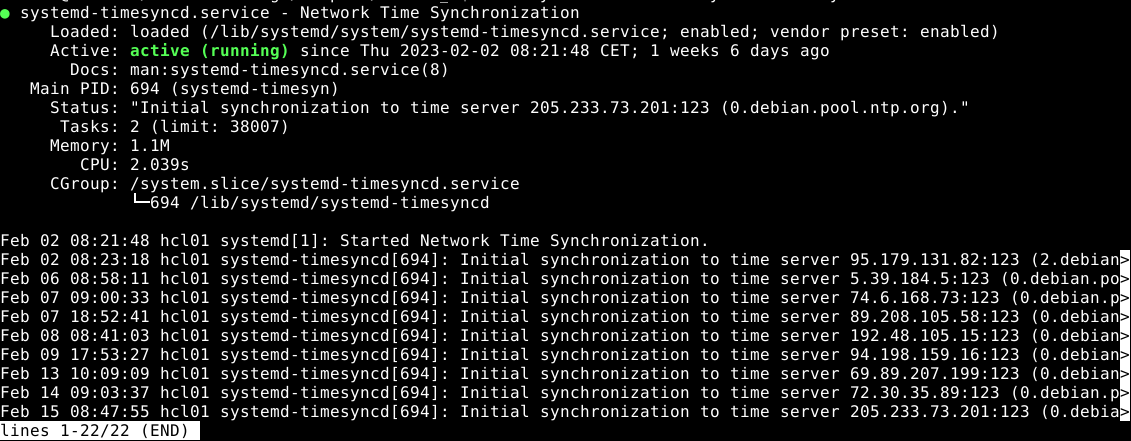
\includegraphics[width=8cm]{systemd-timesyncd-status}
\centering
	\caption{Status output van systemctl}
	\label{scrn:systemd-timesyncd-status}
\end{figure}

Als je net als in het voorbeeld (Figuur \ref{scrn:systemd-timesyncd-status}) een lijn hebt met END dan kan je gebruik maken van 'q' om weer op de command-prompt terecht te komen.

Door aan \texttt{systemctl} de commando's stop of start mee te geven kunnen we daemons op ons systeem stoppen en starten. De tijd synchronisatie daemon is op dit moment gestart, dus het eerste wat we kunnen doen is hem stoppen:

\begin{lstlisting}[language=bash]
sudo systemctl stop systemd-timesyncd
\end{lstlisting}

Met \texttt{systemctl status} kunnen nu de status van de daemon zien en dan zien we dat deze gestopt is. Het opnieuw opstarten doen we met start:

\begin{lstlisting}[language=bash]
sudo systemctl start systemd-timesyncd
\end{lstlisting}


\section{Logging}
\subsection{journalctl}
\texttt{systemd}\index{systemd} is het eerste proces (daemon) dat opgestart wordt op een Linux systeem. Het is daarmee de moeder van alle processen. Als er een daemon opgestart moet worden dan wordt dat gedaan via \texttt{systemd}. \texttt{systemd} is dus de plek waar ook in de gaten gehouden kan worden wat er opgestart is en wat niet en daarmee kan \texttt{systemd} een bijzondere inkijk geven in de status van een systeem. Om meer inzicht te krijgen in wat \texttt{systemd} allemaal voorbij heeft zien komen is er een tool met de naam \texttt{journalctl}\index{journalctl}.

Het opstarten van \texttt{journalctl} zonder enige opties of argumenten laat zien wat \texttt{systemd} heeft verzameld sinds het opstarten van het systeem, of sinds de laatste logrotate.

Om alleen de berichten te zien van een specifiek proces kunnen we het volgende commando gebruiken:
\begin{lstlisting}[language=bash]
$ sudo journalctl -f -u systemd-journald
\end{lstlisting}
De \texttt{-f} optie doet hetzelfde als bij \texttt{tail}, het zegt dat de log gevolgd (follow) moet worden. Met \texttt{-u} geef je op welke 'unit' er gemonitord moet worden.


\subsection{syslog}
\subsection{Log rotation}
\section{Je eigen startup script}
Om een service te starten of te stoppen gebruikt \texttt{systemd} bestanden waarin beschreven wordt hoe een service heet en welke commando's er nodig zijn om te starten en stoppen. Deze beschrijving van een service wordt binnen \texttt{systemd} een \textbf{unit} genoemd. Units kan je onder andere terug vinden in de \texttt{/etc/systemd/system} directory. Een voorbeeld van een unit-file in Debian 11 is de \texttt{syslog.service}. Deze ziet er zo uit:

\begin{lstlisting}[language=bash]
[Unit]
Description=System Logging Service
Requires=syslog.socket
Documentation=man:rsyslogd(8)
Documentation=man:rsyslog.conf(5)
Documentation=https://www.rsyslog.com/doc/

[Service]
Type=notify
ExecStart=/usr/sbin/rsyslogd -n -iNONE
StandardOutput=null
Restart=on-failure

# Increase the default a bit in order to allow many simultaneous
# files to be monitored, we might need a lot of fds.
LimitNOFILE=16384

[Install]
WantedBy=multi-user.target
Alias=syslog.service
\end{lstlisting}

Onder het kopje \textbf{Unit} vind je een beschrijving van de service en wat deze nodig heeft om te kunnen werken. Bij \textit{Requires} staat dat \texttt{syslog} een \texttt{syslog.socket} nodig heeft. Voor nu gaan we ervan uit dat het systeem dit oplost. Wij gaan verder naar de \textbf{Service} kop.

Bij \textit{ExecStart} staat het commando dat gebruikt moet worden op de service op te starten. Zoals je kan zien is er geen commando gegeven om de service te stoppen. Een Unix-achtig systeem heeft de \texttt{kill} functie om om te gaan met processen (zie Linux CLI documentatie). Deze kan gebruikt worden door \texttt{systemd} om processen te stoppen. De \textit{Type} met als waarde Notify zegt dat de daemon aan systemd laat weten wanneer het klaar is met opstarten. Dit heeft als voordeel dat als \texttt{systemd} dit signaal krijgt dat het door kan met andere zaken te doen en niet langer hoeft te wachten. Tot slot is er in deze sectie nog de \textit{Restart} optie die we willen behandelen. Het geeft niet aan wat we moeten doen bij een restart, maar wanneer we moeten restarten. In dit geval als \texttt{rsyslogd} crashed of elke andere willekeurig melding van een error geeft dan wordt het proces geherstart.

Alle Unit-files zijn platte tekst bestanden en kunnen dus met een willekeurige editor aangepast worden. Als je een bestand (service) hebt gewijzigd of toegevoegd moet je \texttt{systemctl} vertellen dat er iets nieuws is. Dat doe je met het volgende commando:
\begin{lstlisting}[language=bash]
$ sudo systemctl daemon-reload
\end{lstlisting}
Hierna kan je de nieuwe of aangepaste service stoppen, starten of herstarten met de gewijzigde settings.



\chapter{Linux in een Windows Domain}
\section{SaMBa}

\chapter{Remote access}
%alleen vanaf het management netwerk
\section{SSH}

\chapter{Mailserver}
\section{postfix}

\chapter{LAMP}
LAMP is een afkorting voor Linux, Apache, MySQL, PHP. Het is een veel gebruikte 'stack' voor het opzetten van webservers op het Internet. Linux is hierbij het operating systeem, Apache de webserver, MySQL de database en PHP de taal die ervoor zorgt dat de browser HTML pagina's met content krijgt, ofwel de server-side scripting language.

In de loop van de tijd zijn er veel variaties op deze afkorting gekomen door vervanging van bijvoorbeeld Linux door Windows (WAMP), of door MacOS X (MAMP), maar er kan ook een andere databases gebruikt worden zoals MariaDB dat een vervanging is voor MySQL, maar we zouden bijvoorbeeld ook PostgreSQL kunnen gebruiken (LAPP) of een andere webserver zoals bijvoorbeeld NGINX (waarbij we de E van engine gebruiken) LEMP, en de P kan ook Perl of Phyton zijn. Wij houden het bij de traditionele stack van LAMP maar vervangen MySQL door MariaDB omdat dat op de meeste systemen aanwezig is en bijna volledig compatible is met MySQL.

Apache, MariaDB en PHP vormen samen de Middleware in onze PAAS (Platform As A Service) omgeving.


\section{Apache}
De meest bekende webserver in gebruik op het Internet is de Apache webserver.

Sinds enige tijd is er een webserver die populairder is dan Apache en dat is NGINX die voornamelijk gebruikt wordt in situaties waar performance belangrijk is.

\begin{lstlisting}[language=bash]
$ sudo apt-get install apache2
\end{lstlisting}


\section{MariaDB}
% Extra disk voor DB
\begin{lstlisting}[language=bash]
$ sudo apt-get install mariadb-server mariadb-client
\end{lstlisting}


\section{PHP}
\begin{lstlisting}[language=bash]
$ sudo apt-get install php
\end{lstlisting}



\chapter{NextCloud}
% Extra disk voor Data
Je mobiele telefoon synchroniseert zijn data met de cloud. De meeste cloud oplossingen draaien op Linux, maar wat is dat nu eigenlijk; de cloud? Letterlijk betekent cloud wolk en dat is ook waar de term vandaan komt, in tekeningen van computer netwerken wordt een totaal netwerk vaak vervangen door een wolkje. Zoals bijvoorbeeld het Internet.

\begin{figure}
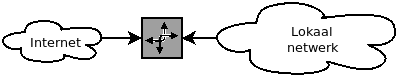
\includegraphics[width=0.99\linewidth]{Cloud_Internet.png}
\end{figure}

De cloud gaat dan ook over diensten die aangeboden worden in een netwerk waarbij het niet meer van belang is op welke machine de data staat, de data bevindt zich ergens in de wolk. Natuurlijk zijn er op de achtergrond fysieke machines waarop de data terecht komt en die beheert moeten worden. In dit hoofdstuk gaan we een machine inrichten met NextCloud. NextCloud is een stukje software geschreven in PHP dat je de mogelijkheid geeft om thuis een cloud systeem te bouwen. Het kan draaien op \'e\'en server met een paar gebruikers en lijkt dan ook heel erg op een NAS (Network Attached Storage) of je kan er een complete cloud dienst mee ontwikkelen dat 100K+ gebruikers ondersteunt zodat het werkt als DropBox of Google Drive. Wij zullen een simpele installatie doen op een enkele (virtuele) machine.

Een NAS gebruikt meestal FTP of SMB om bestanden te delen, Cloud systemen gebruiken het HTTP(s) protocol om via bijvoorbeeld WebDAV data te delen. Dat hoeven niet alleen bestanden te zijn, dat kan ook calender informatie (CalDAV) of adresgegevens (CardDAV) zijn. Met NextCloud zou je je telefoon dus volledig kunnen synchroniseren met je eigen server inplaats van met Google\texttrademark\ of Apple\texttrademark.

NextCloud is een voortzetting van het ownCloud project. De ontwikkeling van ownCloud begon in 2010 en het ownCloud bedrijf ownCloud Inc. werd in 2011 opgericht door Markus Rex, Holger Dyroff and Frank Karlitschek. Het project was bedoelt als een open source vervanger van DropBox. In 2016 werd de code van ownCloud door Frank Karlitschek geforked en omgedoopt tot NextCloud. Een belangrijk deel van het ownCloud ontwikkelteam ging mee met Frank. Sinds 2017 groeit de aanhang van NextCloud, terwijl die van ownCloud daalt.

\section{NextCloud installatie}
In het vorige hoofdstuk heb je al kennis gemaakt met LAMP (Linux, Apache, MySQL en PHP), daar gaan we nu verder mee werken. We gaan MySQL vullen met de gegevens die nodig zijn voor NextCloud en we installeren de NextCloud software, wat PHP is, binnen de Apache omgeving. Om te kunnen beginnen moeten we eerst NextCloud downloaden of installeren vanuit de package manager. Niet elke distributie levert NextCloud mee en omdat het belangrijk is dat je een NextCloud systeem goed bij houdt met betrekking tot de security-patches is het aan te raden om de software zelf te downloaden vanaf de website van NextCloud.

Ga naar \url{https://nextcloud.com/} en klik op Get NextCloud en selecteer Download for Server. Op het moment van schrijven is de meest recente versie versie 19.0.1, dus dat versienummer wordt in de rest van dit document gebruikt. Kijk zelf op de pagina van de NextCloud site wat de meest recente versie is en gebruik dat versienummer in de volgende commando's.

\begin{lstlisting}[language=bash]
$ sudo mkdir -p /srv/www/
$ cd /srv/www/
$ sudo wget https://download.nextcloud.com/server/releases/nextcloud-19.0.1.tar.bz2
$ sudo tar jxvf nextcloud-19.0.1.tar.bz2
\end{lstlisting}

Volg verder de aanwijzingen uit het NextCloud installatie document op \url{https://docs.nextcloud.com/server/19/admin_manual/installation/source_installation.html}.


Voeg de extra PHP modules toe die nodig zijn voor NextCloud
\begin{lstlisting}[language=bash]
$ sudo apt-get install php-curl php-gd php-mbstring php-intl php7.3-mysql php7.3-xml php-zip php-bz2
\end{lstlisting}


%%%%%%%%%%%%%%%%%%%%%
%%% Index and End %%%
%%%%%%%%%%%%%%%%%%%%%
%\backmatter
\printindex
\end{document}

%%% Last line %%%
